% Options for packages loaded elsewhere
\PassOptionsToPackage{unicode}{hyperref}
\PassOptionsToPackage{hyphens}{url}
%
\documentclass[
  a4paper,
]{article}
\usepackage{amsmath,amssymb}
\usepackage{lmodern}
\usepackage{iftex}
\ifPDFTeX
  \usepackage[T1]{fontenc}
  \usepackage[utf8]{inputenc}
  \usepackage{textcomp} % provide euro and other symbols
\else % if luatex or xetex
  \usepackage{unicode-math}
  \defaultfontfeatures{Scale=MatchLowercase}
  \defaultfontfeatures[\rmfamily]{Ligatures=TeX,Scale=1}
\fi
% Use upquote if available, for straight quotes in verbatim environments
\IfFileExists{upquote.sty}{\usepackage{upquote}}{}
\IfFileExists{microtype.sty}{% use microtype if available
  \usepackage[]{microtype}
  \UseMicrotypeSet[protrusion]{basicmath} % disable protrusion for tt fonts
}{}
\makeatletter
\@ifundefined{KOMAClassName}{% if non-KOMA class
  \IfFileExists{parskip.sty}{%
    \usepackage{parskip}
  }{% else
    \setlength{\parindent}{0pt}
    \setlength{\parskip}{6pt plus 2pt minus 1pt}}
}{% if KOMA class
  \KOMAoptions{parskip=half}}
\makeatother
\usepackage{xcolor}
\IfFileExists{xurl.sty}{\usepackage{xurl}}{} % add URL line breaks if available
\IfFileExists{bookmark.sty}{\usepackage{bookmark}}{\usepackage{hyperref}}
\hypersetup{
  pdftitle={MATH5714 Linear Regression, Robustness and Smoothing},
  pdfauthor={Jochen Voss},
  hidelinks,
  pdfcreator={LaTeX via pandoc}}
\urlstyle{same} % disable monospaced font for URLs
\usepackage[margin=1in]{geometry}
\usepackage{color}
\usepackage{fancyvrb}
\newcommand{\VerbBar}{|}
\newcommand{\VERB}{\Verb[commandchars=\\\{\}]}
\DefineVerbatimEnvironment{Highlighting}{Verbatim}{commandchars=\\\{\}}
% Add ',fontsize=\small' for more characters per line
\usepackage{framed}
\definecolor{shadecolor}{RGB}{248,248,248}
\newenvironment{Shaded}{\begin{snugshade}}{\end{snugshade}}
\newcommand{\AlertTok}[1]{\textcolor[rgb]{0.94,0.16,0.16}{#1}}
\newcommand{\AnnotationTok}[1]{\textcolor[rgb]{0.56,0.35,0.01}{\textbf{\textit{#1}}}}
\newcommand{\AttributeTok}[1]{\textcolor[rgb]{0.77,0.63,0.00}{#1}}
\newcommand{\BaseNTok}[1]{\textcolor[rgb]{0.00,0.00,0.81}{#1}}
\newcommand{\BuiltInTok}[1]{#1}
\newcommand{\CharTok}[1]{\textcolor[rgb]{0.31,0.60,0.02}{#1}}
\newcommand{\CommentTok}[1]{\textcolor[rgb]{0.56,0.35,0.01}{\textit{#1}}}
\newcommand{\CommentVarTok}[1]{\textcolor[rgb]{0.56,0.35,0.01}{\textbf{\textit{#1}}}}
\newcommand{\ConstantTok}[1]{\textcolor[rgb]{0.00,0.00,0.00}{#1}}
\newcommand{\ControlFlowTok}[1]{\textcolor[rgb]{0.13,0.29,0.53}{\textbf{#1}}}
\newcommand{\DataTypeTok}[1]{\textcolor[rgb]{0.13,0.29,0.53}{#1}}
\newcommand{\DecValTok}[1]{\textcolor[rgb]{0.00,0.00,0.81}{#1}}
\newcommand{\DocumentationTok}[1]{\textcolor[rgb]{0.56,0.35,0.01}{\textbf{\textit{#1}}}}
\newcommand{\ErrorTok}[1]{\textcolor[rgb]{0.64,0.00,0.00}{\textbf{#1}}}
\newcommand{\ExtensionTok}[1]{#1}
\newcommand{\FloatTok}[1]{\textcolor[rgb]{0.00,0.00,0.81}{#1}}
\newcommand{\FunctionTok}[1]{\textcolor[rgb]{0.00,0.00,0.00}{#1}}
\newcommand{\ImportTok}[1]{#1}
\newcommand{\InformationTok}[1]{\textcolor[rgb]{0.56,0.35,0.01}{\textbf{\textit{#1}}}}
\newcommand{\KeywordTok}[1]{\textcolor[rgb]{0.13,0.29,0.53}{\textbf{#1}}}
\newcommand{\NormalTok}[1]{#1}
\newcommand{\OperatorTok}[1]{\textcolor[rgb]{0.81,0.36,0.00}{\textbf{#1}}}
\newcommand{\OtherTok}[1]{\textcolor[rgb]{0.56,0.35,0.01}{#1}}
\newcommand{\PreprocessorTok}[1]{\textcolor[rgb]{0.56,0.35,0.01}{\textit{#1}}}
\newcommand{\RegionMarkerTok}[1]{#1}
\newcommand{\SpecialCharTok}[1]{\textcolor[rgb]{0.00,0.00,0.00}{#1}}
\newcommand{\SpecialStringTok}[1]{\textcolor[rgb]{0.31,0.60,0.02}{#1}}
\newcommand{\StringTok}[1]{\textcolor[rgb]{0.31,0.60,0.02}{#1}}
\newcommand{\VariableTok}[1]{\textcolor[rgb]{0.00,0.00,0.00}{#1}}
\newcommand{\VerbatimStringTok}[1]{\textcolor[rgb]{0.31,0.60,0.02}{#1}}
\newcommand{\WarningTok}[1]{\textcolor[rgb]{0.56,0.35,0.01}{\textbf{\textit{#1}}}}
\usepackage{longtable,booktabs,array}
\usepackage{calc} % for calculating minipage widths
% Correct order of tables after \paragraph or \subparagraph
\usepackage{etoolbox}
\makeatletter
\patchcmd\longtable{\par}{\if@noskipsec\mbox{}\fi\par}{}{}
\makeatother
% Allow footnotes in longtable head/foot
\IfFileExists{footnotehyper.sty}{\usepackage{footnotehyper}}{\usepackage{footnote}}
\makesavenoteenv{longtable}
\usepackage{graphicx}
\makeatletter
\def\maxwidth{\ifdim\Gin@nat@width>\linewidth\linewidth\else\Gin@nat@width\fi}
\def\maxheight{\ifdim\Gin@nat@height>\textheight\textheight\else\Gin@nat@height\fi}
\makeatother
% Scale images if necessary, so that they will not overflow the page
% margins by default, and it is still possible to overwrite the defaults
% using explicit options in \includegraphics[width, height, ...]{}
\setkeys{Gin}{width=\maxwidth,height=\maxheight,keepaspectratio}
% Set default figure placement to htbp
\makeatletter
\def\fps@figure{htbp}
\makeatother
\setlength{\emergencystretch}{3em} % prevent overfull lines
\providecommand{\tightlist}{%
  \setlength{\itemsep}{0pt}\setlength{\parskip}{0pt}}
\setcounter{secnumdepth}{5}
\ifLuaTeX
  \usepackage{selnolig}  % disable illegal ligatures
\fi
\usepackage[]{natbib}
\bibliographystyle{plainnat}

\title{MATH5714 Linear Regression, Robustness and Smoothing}
\author{\href{mailto:J.Voss@leeds.ac.uk}{Jochen Voss}}
\date{University of Leeds, Semester 1, 2021--22}

\usepackage{amsthm}
\newtheorem{theorem}{Theorem}[section]
\newtheorem{lemma}{Lemma}[section]
\newtheorem{corollary}{Corollary}[section]
\newtheorem{proposition}{Proposition}[section]
\newtheorem{conjecture}{Conjecture}[section]
\theoremstyle{definition}
\newtheorem{definition}{Definition}[section]
\theoremstyle{definition}
\newtheorem{example}{Example}[section]
\theoremstyle{definition}
\newtheorem{exercise}{Exercise}[section]
\theoremstyle{definition}
\newtheorem{hypothesis}{Hypothesis}[section]
\theoremstyle{remark}
\newtheorem*{remark}{Remark}
\newtheorem*{solution}{Solution}
\begin{document}
\maketitle

{
\setcounter{tocdepth}{2}
\tableofcontents
}
\newcommand{\CN}{\mathcal{N}}
\newcommand{\CU}{\mathcal{U}}
\newcommand{\E}{\mathbb{E}}
\newcommand{\argmin}{\mathop{\mathrm{arg\,min}}\limits}
\newcommand{\eps}{\varepsilon}
\newcommand{\R}{\mathbb{R}}
\newcommand{\Var}{\mathop{\mathrm{Var}}}

\hypertarget{home}{%
\section*{Preface}\label{home}}
\addcontentsline{toc}{section}{Preface}

From previous modules we know how to fit a regression line through
points \((x_1, y_1), \ldots, (x_n, y_n) \in\mathbb{R}^2\). The underlying model
here is described by the equation
\begin{equation*}
  y_i
  = \alpha + \beta x_i + \varepsilon_i
\end{equation*}
for all \(i \in \{1, 2, \ldots, n\}\), and the aim is to find values for
the intercept \(\alpha\) and the slope \(\beta\) such that the residuals
\(\varepsilon_i\) are as small as possible. This procedure,
linear regression, and its extensions are discussed in the \href{https://seehuhn.github.io/MATH3714/}{level 3
component of the module}.

In the level 5 component of this module, we will discuss ``smoothing''
which is a technique which can be used when linear models are no longer
appropriate for the data. An example of such a situation is illustrated
in figure~\ref{fig:accel}.



\begin{figure}

{\centering 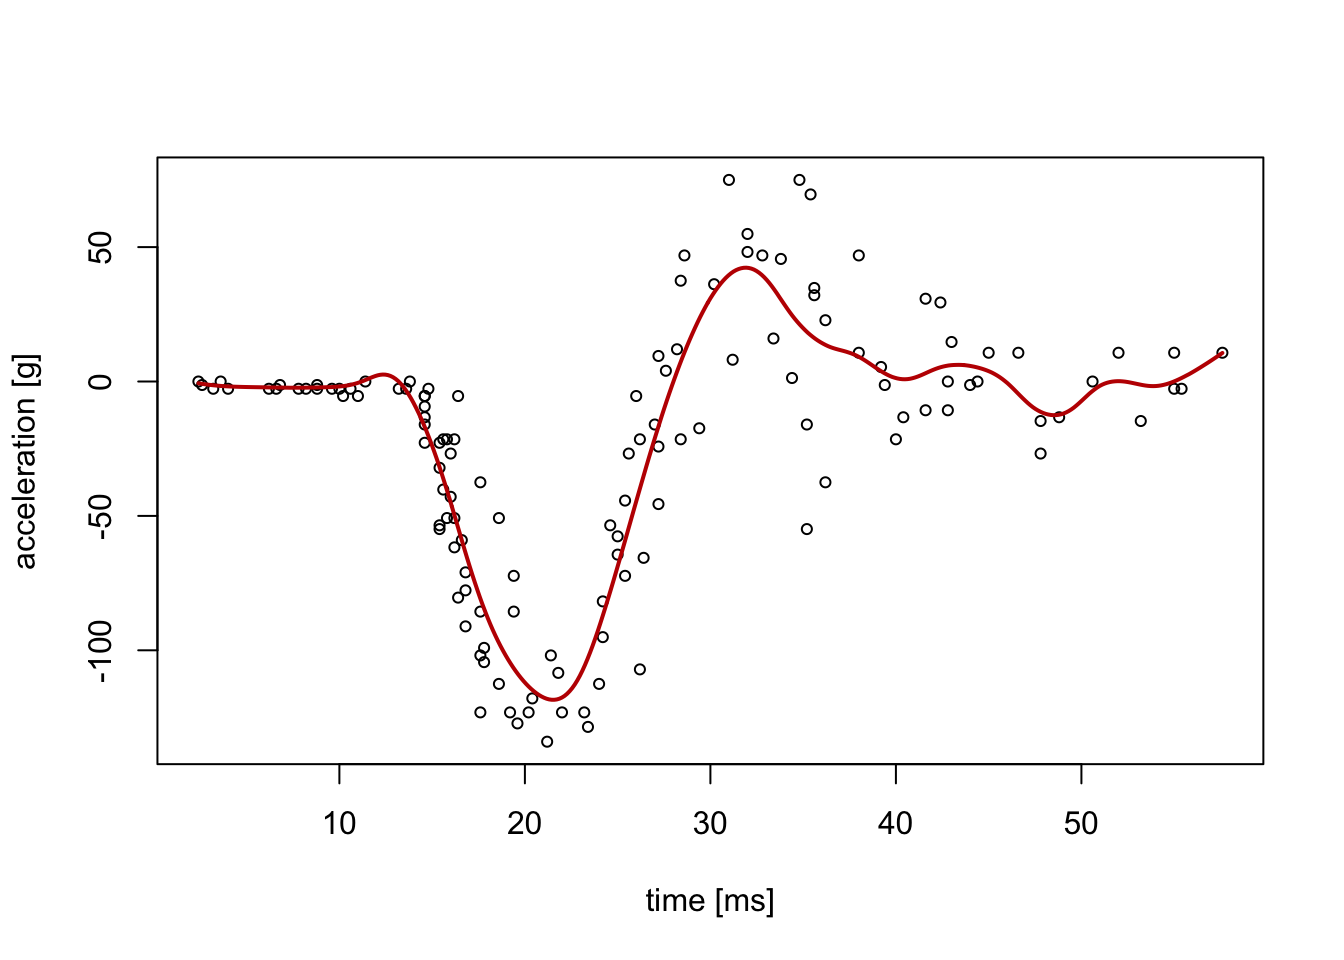
\includegraphics{MATH5714_files/figure-latex/accel-1} 

}

\caption{An illustration of a data set where a linear (straight line) model is not appropriate. The data represents a series of measurements of head acceleration in a simulated motorcycle accident, used to test crash helmets (the \texttt{mcycle} dataset from the \texttt{MASS} R package).}\label{fig:accel}
\end{figure}

\hypertarget{X01-KDE}{%
\section{Kernel Density Estimation}\label{X01-KDE}}

In this section we discuss the topic of ``Kernel Density Estimation''.
Here we suppose we are given data \(x_1,\ldots, x_n \in\mathbb{R}^d\) from an
unknown probability density, say \(f\). Our objective is to estimate
the density~\(f\). This section lays the foundations for many of the
following topics.

\hypertarget{histograms}{%
\subsection{Histograms}\label{histograms}}

\hypertarget{probability-densities}{%
\subsubsection{Probability Densities}\label{probability-densities}}

Before we consider how to estimate a density, let just remember what a
density is. A random variable \(X \in \mathbb{R}\) has \textbf{density} \(f\colon \mathbb{R}\to [0, \infty)\) if
\begin{equation*}
  P\bigl(X \in [a,b]\bigr)
  = \int_a^b f(x) \,dx
\end{equation*}
for all \(a, b\in\mathbb{R}\) with \(a < b\). Densities are sometimes also called
``probability densities'' or even ``probability density functions''.

A density \(f\) is large in regions where \(X\) is very likely to take
values, and small in regions where \(X\) is less likely to take values.
If \(f(x) = 0\) for all \(x\) in a region, that means that \(X\) never takes
values there. Graphically, the integral \(\int_a^b f(x) \,dx\) can be
interpreted as the area under the graph of~\(f\). This is illustrated
in figure~\ref{fig:density}.



\begin{figure}

{\centering 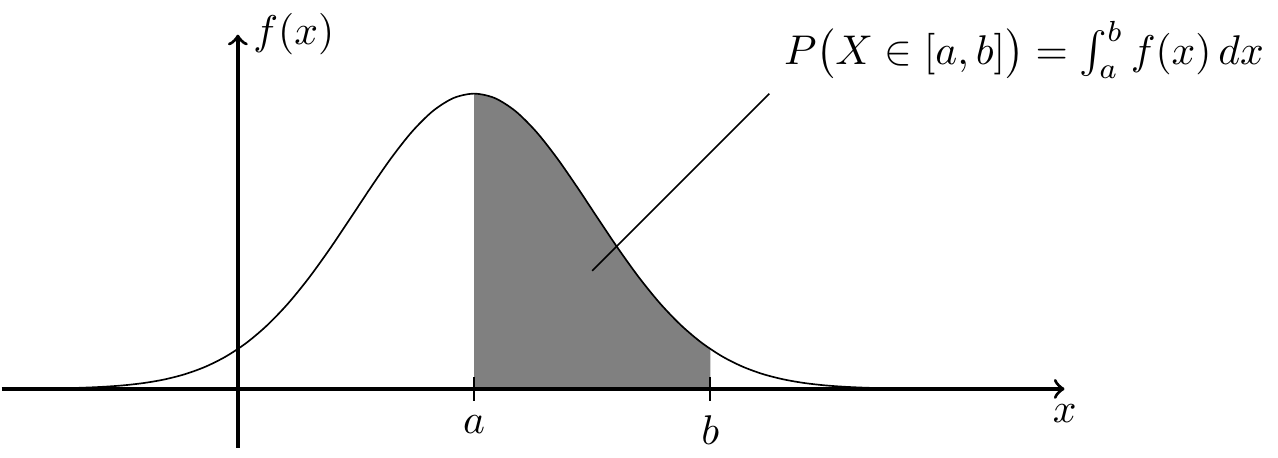
\includegraphics{MATH5714_files/figure-latex/density-1} 

}

\caption{An illustration of how the area under the graph of a density can be interpreted as a probability.}\label{fig:density}
\end{figure}

A function \(f\) is the density of some random variable~\(X\),
if and only if \(f \geq 0\) and
\begin{equation*}
  \int_{-\infty}^\infty f(x) \,dx = 1.
\end{equation*}

\hypertarget{histograms-1}{%
\subsubsection{Histograms}\label{histograms-1}}

In the univariate case, \emph{i.e.}~for \(d = 1\), a commonly used technique
to approximate density of a sample is to plot a histogram. To
illustrate this, we use the \texttt{faithful} dataset built in R, which
contains waiting times between eruptions and the duration of the
eruption for the Old Faithful geyser in the Yellowstone National Park.
(You can type \texttt{help(faithful)} in R to learn more about this data
set.) Here we focus on the waiting times only. A simple histogram
for this dataset is shown in figure~\ref{fig:hist}.



\begin{Shaded}
\begin{Highlighting}[]
\NormalTok{x }\OtherTok{\textless{}{-}}\NormalTok{ faithful}\SpecialCharTok{$}\NormalTok{waiting}
\FunctionTok{hist}\NormalTok{(x, }\AttributeTok{probability =} \ConstantTok{TRUE}\NormalTok{,}
     \AttributeTok{main =} \ConstantTok{NULL}\NormalTok{, }\AttributeTok{xlab =} \StringTok{"time between eruptions [mins]"}\NormalTok{)}
\end{Highlighting}
\end{Shaded}

\begin{figure}
\centering
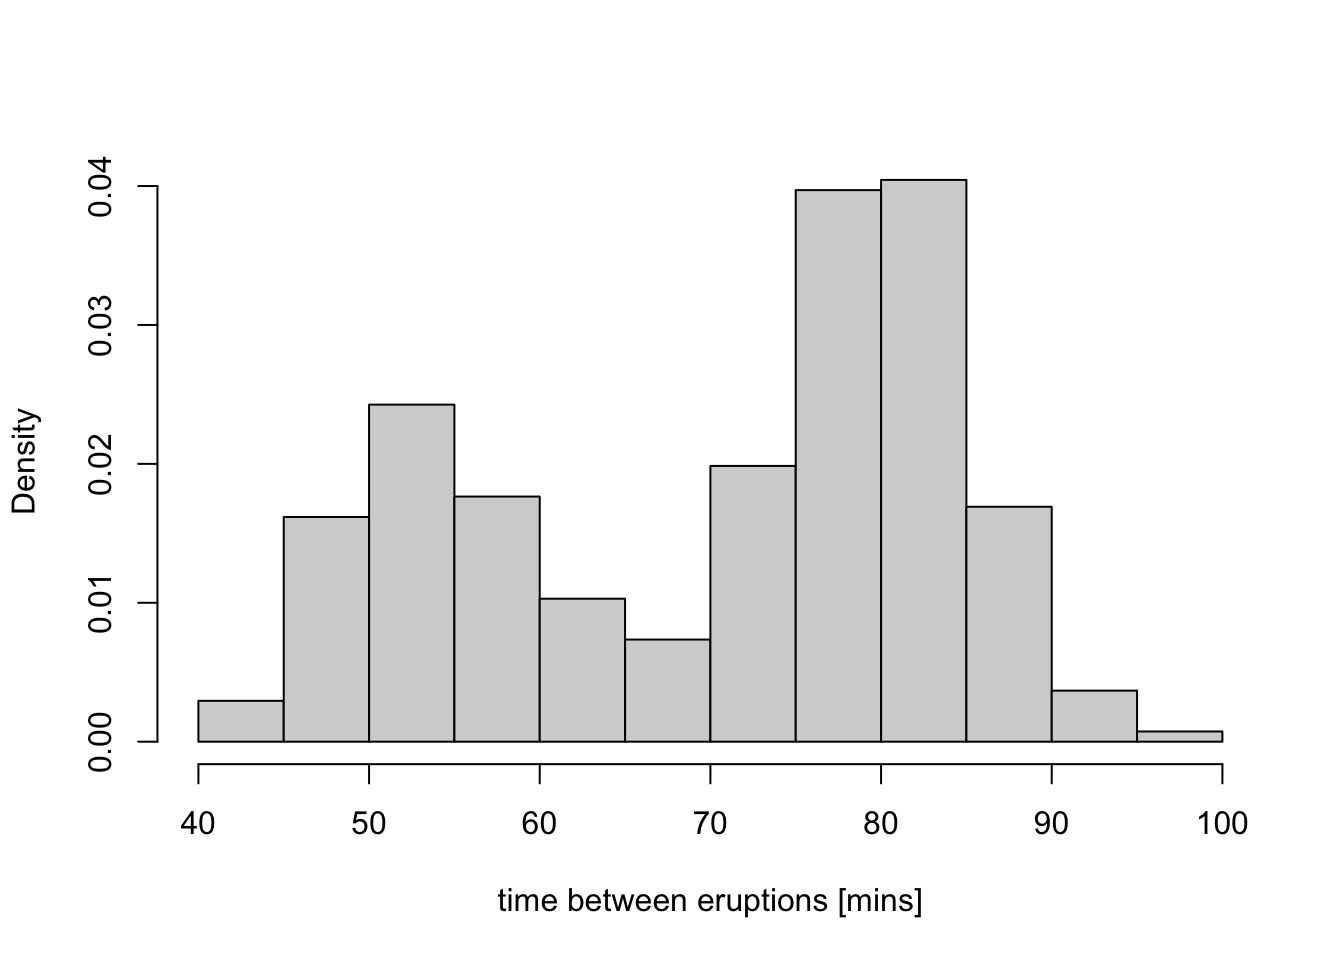
\includegraphics{MATH5714_files/figure-latex/hist-1.pdf}
\caption{\label{fig:hist}This figure shows how a histogram can be used to approximate a probability density. From the plot one can see that the density of the waiting times distribution seems to be bi-modal with peaks around 53 and 80 minutes.}
\end{figure}

The histograms splits the range of the data into ``buckets'', and for
every bucket \([a, b]\) it shows a bar where the height is proportional
the number of samples in the bucket. I am ignoring the case that a
sample may fall exactly on the boundary between two buckets here; in
reality all but one buckets need to be half-open intervals, for
example \([40, 45]\), \((45, 50]\), \ldots, \((95, 100]\).

As we have seen, the area under the graph of the density \(f\) over the
interval \([a, b]\) corresponds to the probability~\(P\bigl(X \in [a,b]\bigr)\). For the histogram to approximate the density, we need
to scale the height \(h_{a,b}\) of the bucket \([a, b]\) so that the area
in the histogram is also close to this probability. Since we don't
know the probability \(P\bigl(X \in [a,b]\bigr)\) exactly, we have to
approximate it as
\begin{equation*}
  P\bigl(X \in [a,b]\bigr)
  \approx \frac{n_{a,b}}{n},
\end{equation*}
where \(n_{a,b}\) is the number of samples in the bucket \([a,b]\),
and \(n\) is the total number of samples. So we need
\begin{align*}
  (b-a) \cdot h_{a,b}
    &= \mbox{area of the histogram bar} \\
    &\approx \mbox{area of the density} \\
    &= P\bigl(X \in [a,b]\bigr) \\
    &\approx \frac{n_{a,b}}{n}.
\end{align*}
and thus we choose
\begin{equation*}
  h_{a,b}
  = \frac{1}{(b - a) n} n_{a,b}.
\end{equation*}
As expected, the height of the bar for the bucket \([a,b]\) is proportional
to the number \(n_{a,b}\) of samples in the bucket.

\hypertarget{choice-of-buckets}{%
\subsubsection{Choice of Buckets}\label{choice-of-buckets}}

Histograms are only meaningful if the buckets are chosen well. If
the buckets are too large, not much of the structure of \(f\) can be
resolved. If the buckets are too small, the estimate \(P\bigl(X \in [a,b]\bigr) \approx n_{a,b}/n\) will be poor and the histogram will
no longer resemble the shape of~\(f\). This



\begin{Shaded}
\begin{Highlighting}[]
\FunctionTok{set.seed}\NormalTok{(}\DecValTok{1}\NormalTok{)}
\NormalTok{x }\OtherTok{\textless{}{-}} \FunctionTok{rnorm}\NormalTok{(}\DecValTok{50}\NormalTok{)}
\FunctionTok{hist}\NormalTok{(x, }\AttributeTok{probability =} \ConstantTok{TRUE}\NormalTok{, }\AttributeTok{main =} \ConstantTok{NULL}\NormalTok{,}
     \AttributeTok{breaks =} \FunctionTok{seq}\NormalTok{(}\SpecialCharTok{{-}}\FloatTok{2.5}\NormalTok{, }\FloatTok{2.5}\NormalTok{, }\AttributeTok{length.out =} \DecValTok{500}\NormalTok{))}
\end{Highlighting}
\end{Shaded}

\begin{figure}
\centering
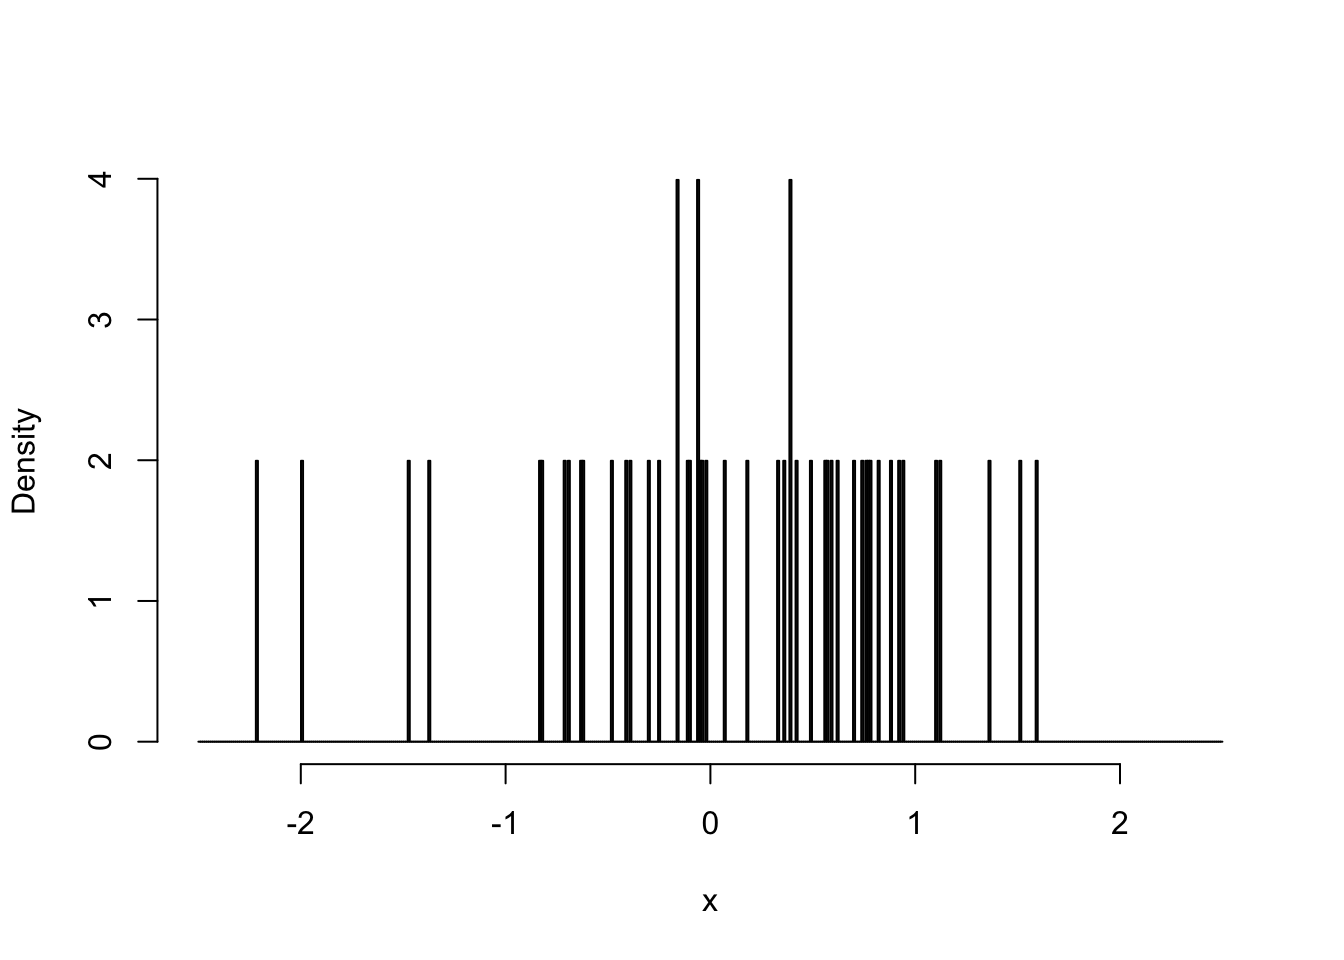
\includegraphics{MATH5714_files/figure-latex/broken-hist-1.pdf}
\caption{\label{fig:broken-hist}This figure shows how a histogram can be used to approximate a probability density. From the plot one can see that the density of the waiting times distribution seems to be bi-modal with peaks around 53 and 80 minutes.}
\end{figure}

Finally, even if reasonable bucket sizes are chosen, the result can
depend quite strongly on the exact locations of these buckets. To illustrate
this effect, we consider a
(dataset about the annual amount of snow){[}\url{https://teaching.seehuhn.de/data/buffalo/}{]}
falling in Buffalo, New York for different years. Figures \ref{fig:buffalo1}
and~\ref{fig:buffalo2} show that same data in two different ways,
allowing to come to different conclusions about the distribution.



\begin{Shaded}
\begin{Highlighting}[]
\CommentTok{\# downloaded from https://teaching.seehuhn.de/data/buffalo/}
\NormalTok{x }\OtherTok{\textless{}{-}} \FunctionTok{read.csv}\NormalTok{(}\StringTok{"data/buffalo.csv"}\NormalTok{)}
\NormalTok{snowfall }\OtherTok{\textless{}{-}}\NormalTok{ x}\SpecialCharTok{$}\NormalTok{snowfall}
\FunctionTok{hist}\NormalTok{(snowfall, }\AttributeTok{probability =} \ConstantTok{TRUE}\NormalTok{,}
     \AttributeTok{breaks =} \FunctionTok{seq}\NormalTok{(}\FloatTok{24.30}\NormalTok{, }\FloatTok{208.22}\NormalTok{, }\AttributeTok{length.out =} \DecValTok{20}\NormalTok{),}
     \AttributeTok{main =} \ConstantTok{NULL}\NormalTok{, }\AttributeTok{xlab =} \StringTok{"snowfall [in]"}\NormalTok{)}
\end{Highlighting}
\end{Shaded}

\begin{figure}
\centering
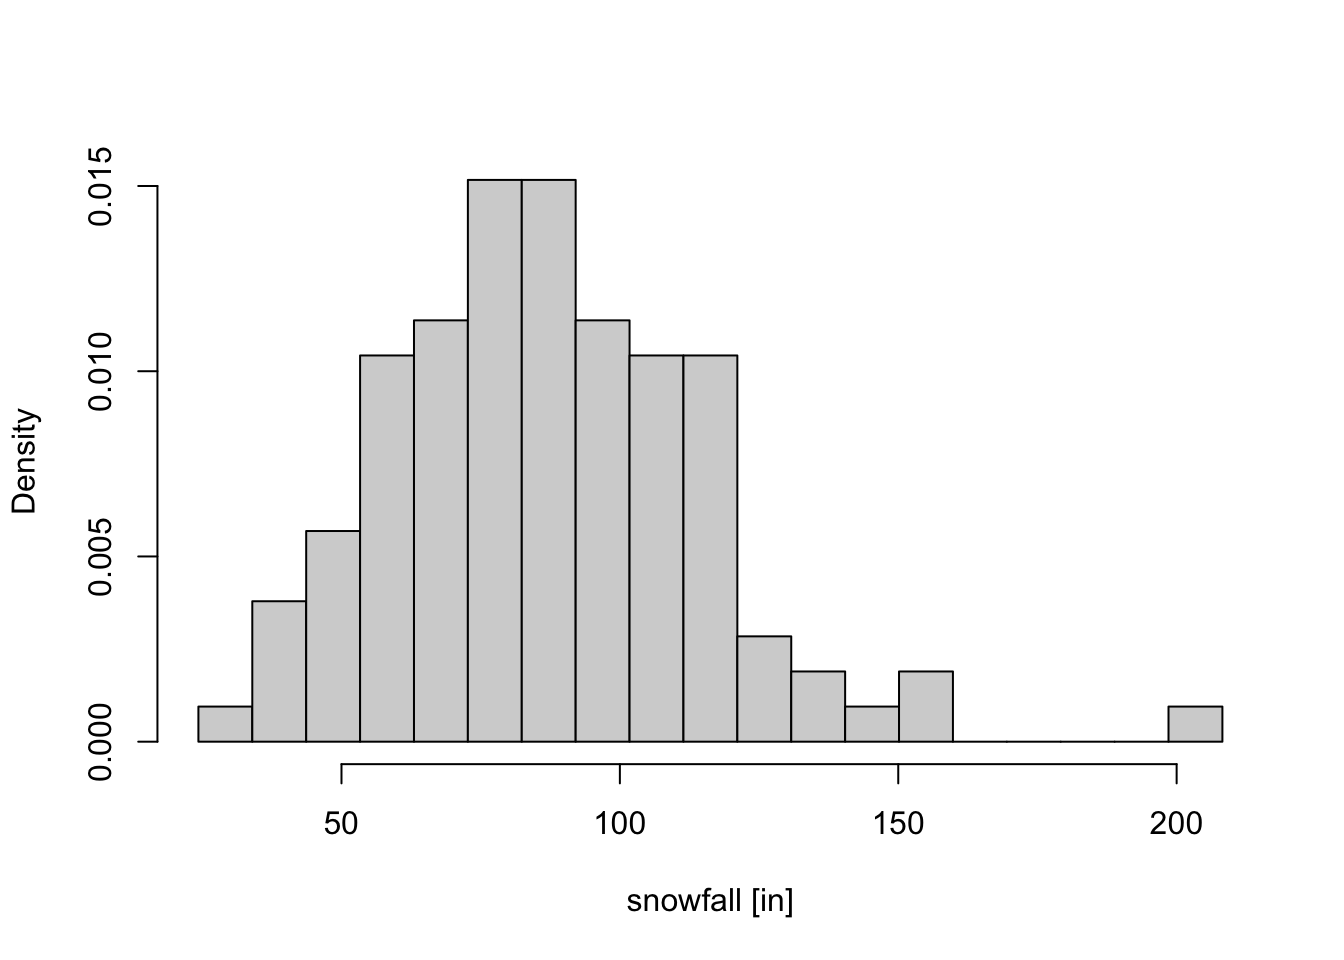
\includegraphics{MATH5714_files/figure-latex/buffalo1-1.pdf}
\caption{\label{fig:buffalo1}The annual amount of snowfall in Buffalo, New York, in inches. The histogram makes it plausible that there is one main peak in the distribution.}
\end{figure}



\begin{Shaded}
\begin{Highlighting}[]
\FunctionTok{hist}\NormalTok{(snowfall, }\AttributeTok{probability =} \ConstantTok{TRUE}\NormalTok{,}
     \AttributeTok{breaks =} \FunctionTok{seq}\NormalTok{(}\FloatTok{22.85}\NormalTok{, }\FloatTok{204.92}\NormalTok{, }\AttributeTok{length.out =} \DecValTok{20}\NormalTok{),}
     \AttributeTok{main =} \ConstantTok{NULL}\NormalTok{, }\AttributeTok{xlab =} \StringTok{"snowfall [in]"}\NormalTok{)}
\end{Highlighting}
\end{Shaded}

\begin{figure}
\centering
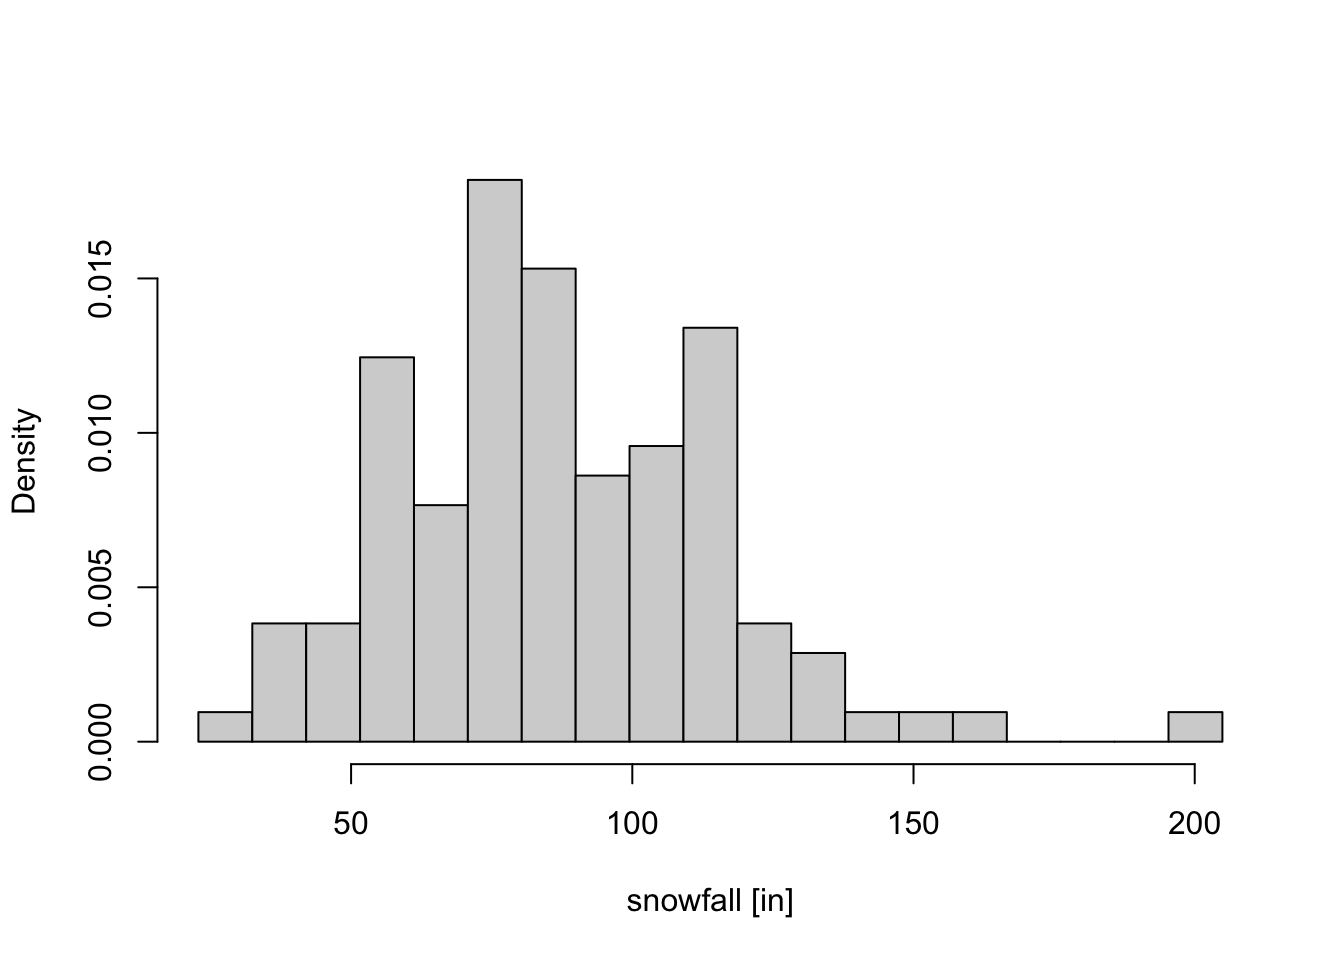
\includegraphics{MATH5714_files/figure-latex/buffalo2-1.pdf}
\caption{\label{fig:buffalo2}Continued from \ref{fig:buffalo1}, this histogram shows the dataset in a way that three peaks are visible.}
\end{figure}

As a further illustration of the effect of bucket width, the code in
figure~\ref{fig:snow-hist-col} shows how histograms with different
bucket widths can be generated in~R. Here we simply specify numeric
values for the \texttt{break} argument to \texttt{hist()}, which R uses as the
\emph{approximate} number of buckets in the plot.



\begin{Shaded}
\begin{Highlighting}[]
\FunctionTok{par}\NormalTok{(}\AttributeTok{mfrow =} \FunctionTok{c}\NormalTok{(}\DecValTok{2}\NormalTok{,}\DecValTok{2}\NormalTok{))}

\ControlFlowTok{for}\NormalTok{ (breaks }\ControlFlowTok{in} \FunctionTok{list}\NormalTok{(}\DecValTok{80}\NormalTok{, }\DecValTok{40}\NormalTok{, }\DecValTok{20}\NormalTok{, }\DecValTok{10}\NormalTok{)) \{}
  \FunctionTok{hist}\NormalTok{(snowfall,}
       \AttributeTok{prob =} \ConstantTok{TRUE}\NormalTok{,}
       \AttributeTok{breaks =}\NormalTok{ breaks,}
       \AttributeTok{xlim =} \FunctionTok{c}\NormalTok{(}\DecValTok{25}\NormalTok{,}\DecValTok{200}\NormalTok{),}
       \AttributeTok{ylim =} \FunctionTok{c}\NormalTok{(}\DecValTok{0}\NormalTok{, }\FloatTok{0.03}\NormalTok{),}
       \AttributeTok{xlab =} \FunctionTok{paste}\NormalTok{(}\StringTok{"breaks ="}\NormalTok{, breaks),}
       \AttributeTok{main =} \ConstantTok{NULL}\NormalTok{)}
\NormalTok{\}}
\end{Highlighting}
\end{Shaded}

\begin{figure}
\centering
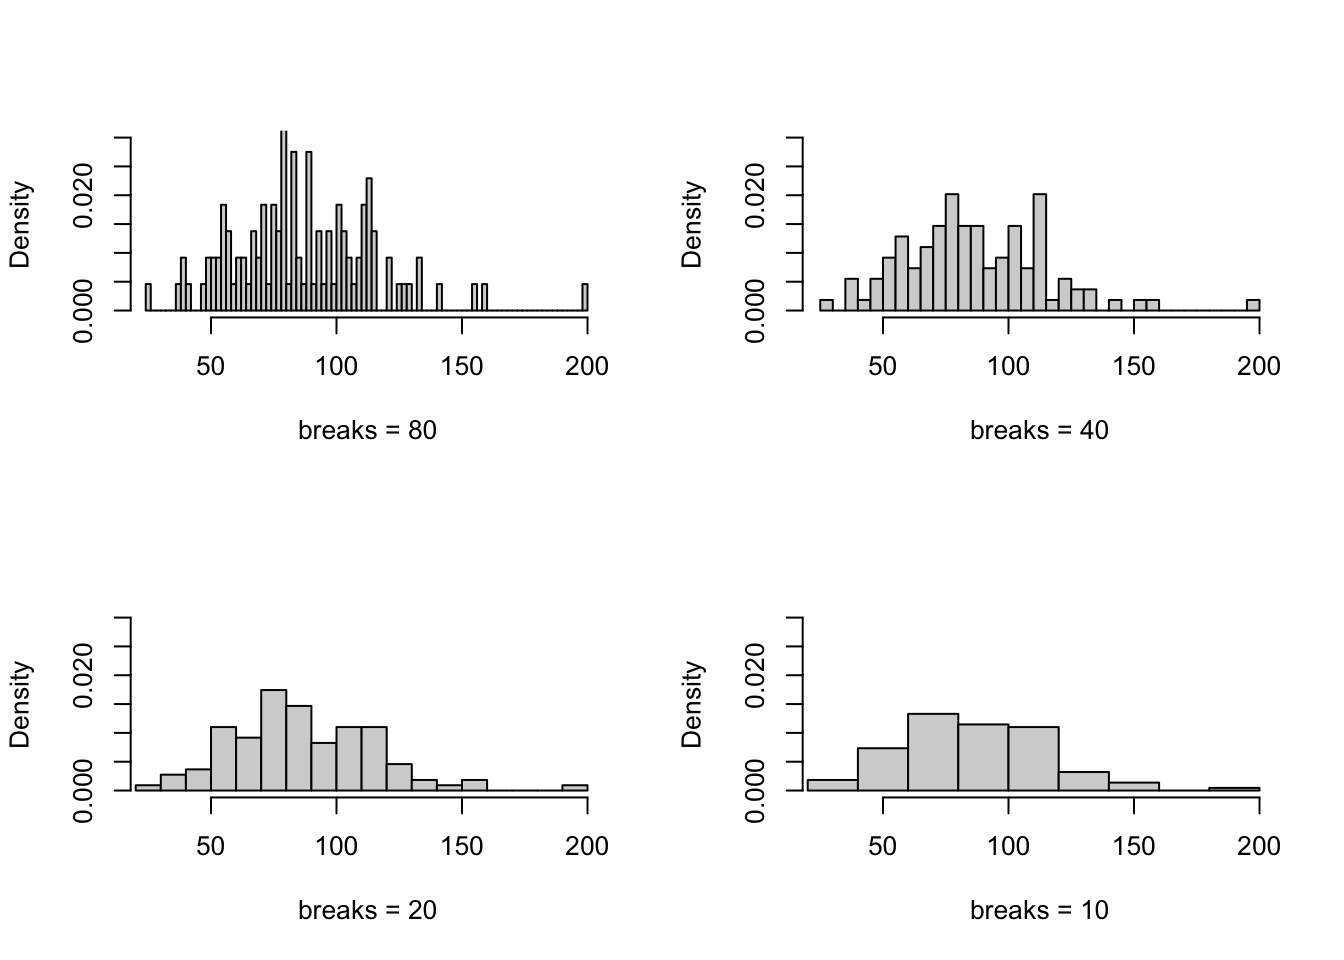
\includegraphics{MATH5714_files/figure-latex/snow-hist-col-1.pdf}
\caption{\label{fig:snow-hist-col}This figure illustrates how the bucket size in a histogram can be controlled in R.}
\end{figure}

\hypertarget{kernel-density-estimation}{%
\subsection{Kernel Density Estimation}\label{kernel-density-estimation}}

Kernel density estimation allows to estimate the density \(f\) for given
data while avoiding some of the disadvantages of histograms.
Again, we suppose that we are given data \(x_1, \ldots, x_n \in \mathbb{R}\)
and that we want to estimate the density \(f\).

\hypertarget{motivation}{%
\subsubsection{Motivation}\label{motivation}}

Similar to the argument in the previous subsection, for \(x\) in a ``small''
interval \([a,b]\) we can estimate \(f(x)\) as
\begin{equation*}
  f(x)
  \approx \frac{1}{b-a} \int_a^b f(y) \,dy
  = \frac{1}{b-a} P\bigl( X\in [a,b] \bigr)
  \approx \frac{1}{b-a} \frac{n_{a,b}}{n},
\end{equation*}
where \(n_{a,b}\) denotes the number of samples in the interval \([a, b]\).
This equation contains two approximation. The first one,
\(f(x) \approx 1/(ba) \int_a^b f(y) \,dy\), is more accurate if the
interval is small, because then \(f\) will be nearly constant over the
interval. The second approximation will be more accurate if the
interval is large, because then the interval \([a,b]\) covers more samples
and the estimate of the probability is based on more data. We will later
discuss in detail how these two concerns can be optimally balanced.

A mathematical ``trick'' to write more clearly how \(n_{a,b}\) depends on the
data is to write the value as
\begin{equation*}
  n_{a,b}
  = \sum_{i=1}^n I_{[a,b]}(x_i),
\end{equation*}
where
\begin{equation*}
  I_{[a,b]}(x)
  = \begin{cases}
    1 & \mbox{if $x \in [a,b]$, and} \\
    0 & \mbox{otherwise.}
  \end{cases}
\end{equation*}
The function \(I_{[a,b]}\) is called the \textbf{indicator function} of the
set~\([a, b]\).

Using the indicator function notation, the estimate for \(f(x)\)
can be written as
\begin{align*}
  f(x)
  \approx \frac{1}{n(b-a)} n_{a,b}
  = \frac{1}{n} \sum_{i=1}^n \frac{1}{b-a} I_{[a,b]}(x_i)
\end{align*}
whenever \(x \in [a,b]\) and when \(b-a\) is ``not too large and not too small''.
For symmetry we choose the interval \([a, b]\) centred around \(x\),
say \([a, b] = [x - h, x + h]\) where \(h\) can be chosen to control the
width of the interval. In this case we have \(b - a = x + h - x + h = 2h\) and thus
\begin{align*}
  f(x)
  &\approx \frac{1}{n} \sum_{i=1}^n \frac{1}{2h} I_{[x-h,x+h]}(x_i) \\
  &= \frac{1}{n} \sum_{i=1}^n \frac{1}{2h} I_{[-h,+h]}(x_i-x) \\
  &= \frac{1}{n} \sum_{i=1}^n \frac{1}{2h} I_{[-1,+1]}\Bigl(\frac{x_i-x}{h}\Bigr)
\end{align*}
for all \(x \in \mathbb{R}\). This is an example of a kernel density estimate.
The function \(K(x) = 1/2 \, I_{[-1,+1]}(x)\) on the right-hand side is
called the kernel of the estimate, and the parameter \(h\) is called the
\textbf{bandwidth} or the smoothing parameter.

\hypertarget{definition-of-a-kernel-density-estimator}{%
\subsubsection{Definition of a Kernel Density Estimator}\label{definition-of-a-kernel-density-estimator}}

The general kernel density estimate is a generalisation of the idea
from the previous subsection. We first define the class of functions
which we use to replace the function \(1/2 \, I_{[-1,+1]}\).

\begin{definition}
\protect\hypertarget{def:kernel}{}\label{def:kernel}

A \textbf{kernel} is a function \(K\colon \mathbb{R}\to \mathbb{R}\) such that

\begin{itemize}
\tightlist
\item
  \(\int_{-\infty}^\infty K(x) \,dx = 1\),
\item
  \(K(x) \geq 0\), and
\item
  \(K(x) = K(-x)\) for all \(x\in \mathbb{R}\).
\end{itemize}

\end{definition}

Of these three properties, the third one is the most important one.
While most authors list all three properties shown above, sometimes
the second condition and very rarely also the first condition are
omitted. One advantage of including the second condition is, that with
this condition in place, kernel functions are also probability distribution
functions.

It is easy to check that \(K(x) = 1/2 \, I_{[-1,+1]}(x)\) satisfies all
three conditions of definition~\ref{def:kernel}. This function \(K\)
is sometimes called the ``uniform kernel'', because it is the density
of the uniform distribution~\(\mathcal{U}[-1,+1]\).

Based on the concept of a kernel, we now can define
what a Kernel Density Estimate is.

\begin{definition}
\protect\hypertarget{def:KDE}{}\label{def:KDE}For a kernel~\(K\), bandwidth~\(h > 0\) and \(x \in \mathbb{R}\), the
\textbf{kernel density estimate} for \(f(x)\) is given by
\begin{equation*}
  \hat f_h(x)
  = \frac{1}{n} \sum_{i=1}^n K_h(x - x_i),
\end{equation*}
where \(K_h\) is given by
\begin{equation*}
  K_h(y)
  = \frac{1}{h} K(y/h)
\end{equation*}
for all \(y\in \mathbb{R}\).
\end{definition}

For \(K(x) = 1/2 \, I_{[-1,+1]}(x)\) this definition recovers the
approximation we discussed in the previous section. In later sections
we will see how the kernel \(K\) can be chosen for the estimator \(\hat f\) to have ``good'' properties. As a simple example we note that if \(K\)
is continuous, then the rescaled kernel \(K_h\) and thus also the
estimate \(f_h\) are continuous functions.

Similar to the bucket width in histograms, the bandwidth parameter~\(h\)
controls how smooth the density estimate~\(\hat f_h\) is, as a function
of~\(x\).

\hypertarget{kernels}{%
\subsubsection{Kernels}\label{kernels}}

There are many different kernels in use. Some examples are listed
below. A more exhautive list can, for example, be found
\href{https://en.wikipedia.org/wiki/Kernel_(statistics)\#Kernel_functions_in_common_use}{on Wikipedia}.

\hypertarget{uniform-kernel}{%
\paragraph{Uniform Kernel}\label{uniform-kernel}}

\begin{equation*}
  K(x)
  = \begin{cases}
      1/2 & \mbox{if $-1 \leq x \leq 1$} \\
      0 & \mbox{otherwise}
    \end{cases}
\end{equation*}

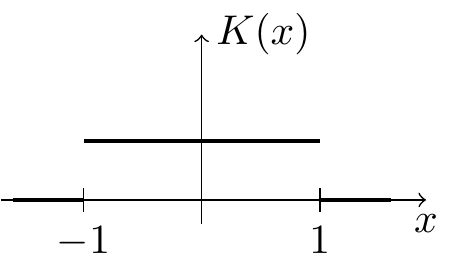
\includegraphics{MATH5714_files/figure-latex/kUniform-1.pdf}

\hypertarget{triangular-kernel}{%
\paragraph{Triangular Kernel}\label{triangular-kernel}}

\begin{equation*}
  K(x)
  = \begin{cases}
      1-|x| & \mbox{if $-1 \leq x \leq 1$} \\
      0 & \mbox{otherwise}
    \end{cases}
\end{equation*}

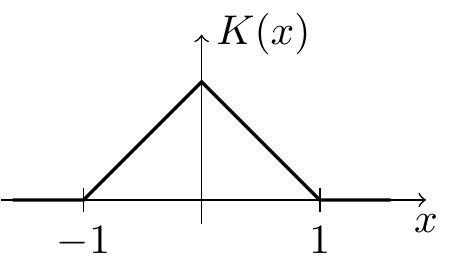
\includegraphics{MATH5714_files/figure-latex/kTriangular-1.pdf}

\hypertarget{epanechnikov-kernel}{%
\paragraph{Epanechnikov Kernel}\label{epanechnikov-kernel}}

\begin{equation*}
  K(x)
  = \begin{cases}
      \frac34 (1-x^2) & \mbox{if $-1 \leq x \leq 1$} \\
      0 & \mbox{otherwise}
    \end{cases}
\end{equation*}

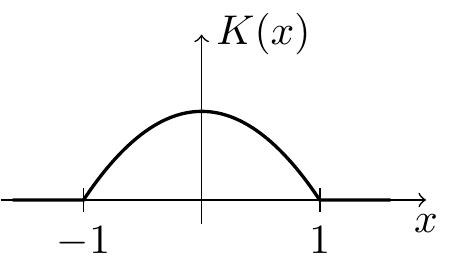
\includegraphics{MATH5714_files/figure-latex/kEpanechnikov-1.pdf}

\hypertarget{gaussian-kernel}{%
\paragraph{Gaussian Kernel}\label{gaussian-kernel}}

\begin{equation*}
  K(x)
  = \frac{1}{\sqrt{2\pi}} \exp\bigl(-x^2/2\bigr)
\end{equation*}

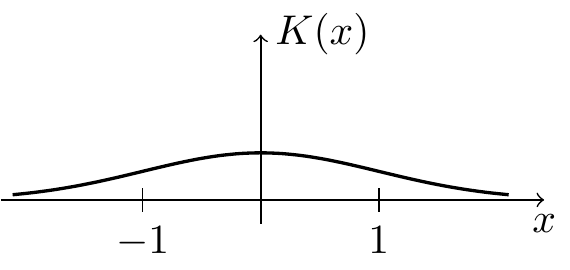
\includegraphics{MATH5714_files/figure-latex/kGaussian-1.pdf}

\hypertarget{kernel-density-estimation-in-r}{%
\subsection{Kernel Density Estimation in R}\label{kernel-density-estimation-in-r}}

Kernel density estimates can be computed in R using the built-in
\texttt{density()} function. If \texttt{x} is a vector containing the data, then
\texttt{density(x)} computes a basic kernel density estimate, using the
Gaussian kernel. The function has a number of optional arguments,
which can be used to control details of the estimate:

\begin{itemize}
\item
  \texttt{bw\ =\ ...} can be used to control the bandwidth~\(h\).
  If no numeric value is given, a heuristic is used.
  Note that for some kernels, \texttt{bw} differs from our \(h\)
  by a constant factor. The value \texttt{bw=1} always corresponds
  to the case where the probability distribution with density
  \(K_h\) has variance~1.
\item
  \texttt{kernel\ =\ ...} can be used to choose the kernel.
  Choices incluse \texttt{"rectangular"} (the uniform kernel), \texttt{"triangular"},
  \texttt{"epanechnikov"} and \texttt{"gaussian"}.
\end{itemize}

Details about how to call \texttt{density()} can be found by using the
command \texttt{help(density)} in R. The help page is also
\href{https://stat.ethz.ch/R-manual/R-devel/library/stats/html/density.html}{available online}.

The return value of \texttt{density} is an R object which contains information
about the kernel density estimate.

\begin{Shaded}
\begin{Highlighting}[]
\NormalTok{m }\OtherTok{\textless{}{-}} \FunctionTok{density}\NormalTok{(snowfall)}
\FunctionTok{str}\NormalTok{(m)}
\end{Highlighting}
\end{Shaded}

\begin{verbatim}
## List of 7
##  $ x        : num [1:512] -4.17 -3.72 -3.26 -2.81 -2.35 ...
##  $ y        : num [1:512] 4.32e-06 4.98e-06 5.73e-06 6.56e-06 7.48e-06 ...
##  $ bw       : num 9.72
##  $ n        : int 109
##  $ call     : language density.default(x = snowfall)
##  $ data.name: chr "snowfall"
##  $ has.na   : logi FALSE
##  - attr(*, "class")= chr "density"
\end{verbatim}

The field \texttt{\$x} and \texttt{\$y} contain the \(x\) and~\(y\) coordinates, respectively,
of points on the \(x \mapsto \hat f_h(x)\) curve, which approximates~\(f\).
The field \texttt{\$bw} shows the numeric value for the bandwidth chosen by
the heuristic. The returned object can also directly be used
as an argument to \texttt{plot()} and \texttt{lines()}, to add the graph of \(\hat f_h\)
to a plot. The commands in figure~\ref{fig:snow-dens-col} show how the
command \texttt{density()} can be used and illustrate the effect of the
bandwidth parameter.



\begin{Shaded}
\begin{Highlighting}[]
\FunctionTok{par}\NormalTok{(}\AttributeTok{mfrow =} \FunctionTok{c}\NormalTok{(}\DecValTok{2}\NormalTok{,}\DecValTok{2}\NormalTok{))}

\ControlFlowTok{for}\NormalTok{ (bw }\ControlFlowTok{in} \FunctionTok{list}\NormalTok{(}\DecValTok{1}\NormalTok{, }\DecValTok{2}\NormalTok{, }\DecValTok{4}\NormalTok{, }\DecValTok{8}\NormalTok{)) \{}
  \FunctionTok{plot}\NormalTok{(}\FunctionTok{density}\NormalTok{(snowfall, }\AttributeTok{bw =}\NormalTok{ bw, }\AttributeTok{kernel =} \StringTok{"triangular"}\NormalTok{, }\AttributeTok{n =} \DecValTok{1000}\NormalTok{),}
    \AttributeTok{xlim =} \FunctionTok{c}\NormalTok{(}\DecValTok{25}\NormalTok{,}\DecValTok{200}\NormalTok{),}
    \AttributeTok{ylim =} \FunctionTok{c}\NormalTok{(}\DecValTok{0}\NormalTok{, }\FloatTok{0.03}\NormalTok{),}
    \AttributeTok{xlab =} \FunctionTok{paste}\NormalTok{(}\StringTok{"bandwidth ="}\NormalTok{, bw),}
    \AttributeTok{main =} \ConstantTok{NA}\NormalTok{)}
\NormalTok{\}}
\end{Highlighting}
\end{Shaded}

\begin{figure}
\centering
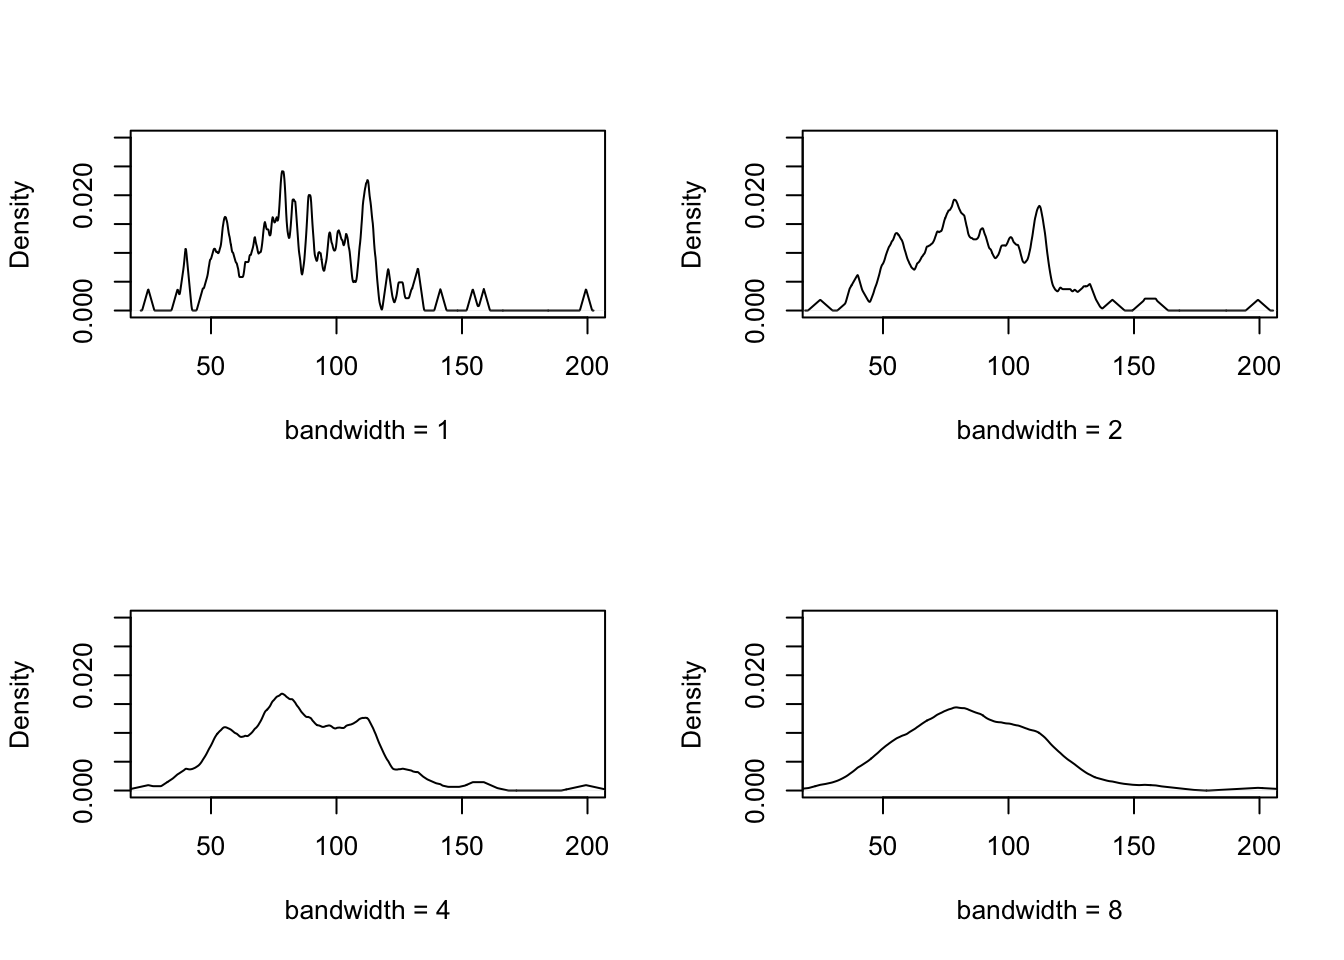
\includegraphics{MATH5714_files/figure-latex/snow-dens-col-1.pdf}
\caption{\label{fig:snow-dens-col}This figure illustrates how the bandwidth of a kernel density estimate can be controlled in R.}
\end{figure}

\textbf{Summary}

\begin{itemize}
\tightlist
\item
  Histograms can be scaled so that they approximate densities.
\item
  Some care is needed when choosing buckets for a histogram.
\item
  Kernel density estimates can be used to estimate densities from data.
\item
  A variety of different kernel functions are commonly used.
\end{itemize}

\end{document}
